\newcommand{\DoNotLoadEpstopdf}{}
\PassOptionsToPackage{hyphens}{url}
\documentclass[11pt]{article}
\usepackage[T1]{fontenc}
\usepackage[utf8]{inputenc}
\usepackage{lmodern}
\usepackage[a4paper,margin=28mm]{geometry}
\usepackage{amsmath,amssymb,amsthm,mathtools}
\usepackage{microtype}
\usepackage{enumitem}
\usepackage{tikz-cd}
\usepackage{xcolor}
\usepackage{hyperref}
\hypersetup{colorlinks=true,linkcolor=blue!45!black,citecolor=blue!45!black,
  urlcolor=blue!45!black,pdftitle={Two-step monodromy of special quasi-projective varieties},pdfauthor={OpenAI}}
\urlstyle{same}
\setlength{\emergencystretch}{2em}
\numberwithin{equation}{section}
\newtheorem{theorem}{Theorem}[section]
\newtheorem{proposition}[theorem]{Proposition}
\newtheorem{lemma}[theorem]{Lemma}
\newtheorem{corollary}[theorem]{Corollary}
\theoremstyle{definition}
\newtheorem{definition}[theorem]{Definition}
\newtheorem{question}[theorem]{Question}
\theoremstyle{remark}
\newtheorem{remark}[theorem]{Remark}
\newcommand{\C}{\mathbf C}
\newcommand{\Q}{\mathbf Q}
\newcommand{\R}{\mathbf R}
\newcommand{\Z}{\mathbf Z}
\newcommand{\PP}{\mathbf P}
\renewcommand{\AA}{\mathbf A}
\newcommand{\Gm}{\mathbf G_m}
\newcommand{\Ga}{\mathbf G_a}
\newcommand{\OO}{\mathcal O}
\newcommand{\g}{\mathfrak g}
\newcommand{\kk}{\mathfrak k}
\newcommand{\m}{\mathfrak m}
\DeclareMathOperator{\Alb}{Alb}
\DeclareMathOperator{\im}{im}
\DeclareMathOperator{\Lie}{Lie}
\DeclareMathOperator{\Tor}{Tor}
\DeclareMathOperator{\codim}{codim}
\DeclareMathOperator{\Bl}{Bl}
\DeclareMathOperator{\GL}{GL}
\DeclareMathOperator{\gr}{gr}
\DeclareMathOperator{\Supp}{Supp}
\DeclareMathOperator{\divisor}{div}
\newcommand{\ab}{\mathrm{ab}}
\newcommand{\un}{\mathrm{un}}
\newcommand{\et}{\mathrm{\acute et}}
\newcommand{\cl}{\overline}
\title{Two-step monodromy of special\protect\\ quasi-projective varieties}
\author{OpenAI}
\date{September 24, 2026}
\begin{document}
\maketitle
\begin{abstract}
We give an independent proof that every complex linear representation
of the ordinary fundamental group of a connected smooth special complex
quasi-projective variety has virtually nilpotent image of class at most
two. This conclusion was previously announced by
Cao--Deng--Hacon--P\u aun. We also construct special open surfaces whose
general quasi-Albanese fibres are not special.
\end{abstract}

\section{Introduction}\label{sec:introduction}

Campana's theory of special varieties relates the absence of fibrations
of general type to restrictions on topology and monodromy
\cite{Campana2004,Campana2011}. Throughout the monodromy statements,
\emph{special} means special in the open-variety convention of
\cite[Definition 2.1]{CDY2025}: after any proper birational modification,
every dominant algebraic fibration with connected general fibre onto a
positive-dimensional normal quasi-projective base has orbifold-base
Kodaira dimension smaller
than the dimension of that base. The orbifold-base Kodaira dimension is
computed birationally,
using infimum multiplicities on smooth compactifications; a removed
divisor has multiplicity infinity. Section~\ref{sec:definitions}
spells out these conventions and the upper-model condition on orbifold
pairs that we verify for our surface example. That pair condition
implies the open-variety condition used here. For a smooth curve
$C=\bar C\setminus B$, specialness is equivalent to
\[
 \deg(K_{\bar C}+B)=2g(\bar C)-2+\#B\leq0.
\]
Thus elliptic curves are special, whereas a projective line with
at least three punctures is not.

In the compact setting, Campana's abelianity conjecture asks for a
virtually abelian ordinary fundamental group
\cite[Conjecture 7.1, p.~595]{Campana2004}. Campana--Claudon proved this
for special compact K\"ahler threefolds
\cite[Theorem 1.3]{CampanaClaudon2014}; the companion
\cite[Theorem 1.1]{OpenAICompactAbelianity2026} proves it in arbitrary
complex dimension. The open setting admits nonabelian nilpotent groups.
Our first result concerns complex linear images of ordinary fundamental
groups in this setting.

For a group $G$, put $\gamma_1G=G$ and
$\gamma_{r+1}G=[G,\gamma_rG]$. It has \emph{nilpotency class at most two}
if $\gamma_3G=1$, equivalently if every commutator is central. A property
holds \emph{virtually} if it holds in a subgroup of finite index.

\begin{theorem}[Two-step linear monodromy]\label{thm:linear}
Let $V$ be a connected smooth special complex quasi-projective variety.
For every positive integer $d$ and every representation
$\rho:\pi_1(V)\to\GL_d(\C)$, the image $\rho(\pi_1(V))$ has a subgroup
of finite index and nilpotency class at most two.
\end{theorem}

Cadorel--Deng--Yamanoi established virtual nilpotence of these linear
images: the identity component of their Zariski closure is a direct
product of a unipotent group and a torus
\cite[Theorem A/4.1]{CDY2025}. Cao--Deng--Hacon--P\u aun subsequently
announced the sharp class-two conclusion of Theorem~\ref{thm:linear}
\cite[Theorem A, equivalently Theorem 6.2]{CDHP2026}. Priority for that
conclusion belongs to their work. We give a different proof from the
independent CDY inputs and a structural theorem about unipotent
completion.

The bound is optimal. Cadorel--Deng--Yamanoi construct a smooth special
quasi-projective surface with a linear, two-step nilpotent fundamental
group that is not virtually abelian
\cite[Example 4.25 and Remarks 4.28--4.29]{CDY2025}. It is the complement
of the zero section in a degree-one line bundle on an elliptic curve;
its group is a Heisenberg central extension. Its ruled compactification
with the zero and infinity sections as reduced boundary has $K+D=0$
\cite[Lemma 5.10]{CDY2025}, and is special also in the orbifold-pair
convention by \cite[arXiv version, Theorem 6.7]{Campana2011}.

\subsection{The structural completion theorem}
A \emph{semiabelian variety} is a connected algebraic group fitting into
an exact sequence
\[
 1\longrightarrow\Gm^r\longrightarrow A\longrightarrow B
 \longrightarrow1,
\]
where $B$ is an abelian variety. For a connected smooth quasi-projective
variety $V$ with a chosen base point, the algebraic
\emph{quasi-Albanese map} $a_V:V\to\Alb(V)$ is the universal based
algebraic morphism to a semiabelian variety. This is the open analogue
of the Albanese map. We use the construction and universal property
recalled by Fujino \cite[Definition 2.18 and Theorem 3.16]{Fujino2024};
universality concerns algebraic morphisms, not arbitrary holomorphic
maps.

The \emph{rational unipotent completion} of a group $\Gamma$ is the
universal pro-unipotent algebraic group receiving a homomorphism from
$\Gamma$. Here pro-unipotent means an inverse limit of unipotent
algebraic groups, and universality means that every homomorphism from
$\Gamma$ to a finite-dimensional unipotent algebraic group over $\Q$
factors uniquely through the completion. For the finitely generated
groups considered here and each integer $c\geq1$, its
\emph{canonical $c$-step quotient} is the universal unipotent
quotient of nilpotency class at most $c$: every homomorphism to a
unipotent algebraic group of class at most $c$ factors uniquely through
it. Section~\ref{sec:mhs} gives its Lie-algebra construction.

\begin{theorem}[Completion under quasi-Albanese exactness]\label{thm:completion}
Let $V$ be a connected smooth complex quasi-projective variety and let
$a:V\to A=\Alb(V)$ be its algebraic quasi-Albanese map. Suppose $a$ is
dominant, choose a smooth connected general fibre $F$ and a point
$v\in F$, and assume that the sequence of ordinary fundamental groups
\begin{equation}\label{eq:exact}
 \pi_1(F,v)\longrightarrow\Gamma:=\pi_1(V,v)
 \xrightarrow{a_*}\Lambda:=\pi_1(A,a(v))\longrightarrow1
\end{equation}
is exact. Then every canonical rational unipotent quotient of $\Gamma$
has nilpotency class at most two. The full rational unipotent completion
is a finite-dimensional unipotent algebraic group of class at most two.
Every finite-dimensional complex unipotent representation of $\Gamma$
also has image of class at most two.
\end{theorem}

Exactness in \eqref{eq:exact} identifies the image of the fibre group
with the whole kernel of $a_*$; the first arrow need not be injective.
The theorem assumes neither specialness of $V$ or $F$ nor initial
nilpotence of the discrete group $\Gamma$. Its geometric hypotheses
are useful because the quasi-Albanese map identifies first homology,
and the algebraic fibre inclusion gives a morphism of pointed mixed
Hodge structures. These two facts connect the actual fibre image to
the commutator of each canonical unipotent quotient.

The proof uses Deligne's mixed Hodge theory for smooth open varieties
\cite{Deligne1971}, Morgan's foundational work on nilpotent homotopy data
\cite{Morgan1978,Morgan1986}, and Hain's canonical pointed construction
\cite{Hain1987}. At each finite stage, let $\g$ be the canonical
nilpotent Lie algebra and $\kk$ the image of the fibre Lie algebra.
Exactness and the quasi-Albanese first-homology isomorphism imply
$\kk=[\g,\g]$. The abelianization of $\kk$ is a quotient of
$H_1(F,\Q)$, with weights $-1$ and $-2$, while its position in a
commutator forces weights at most $-2$. It is therefore pure of weight
$-2$. The conjugation bracket has source of weights at most $-3$, so it
vanishes in this abelianization. This yields
$\gamma_3\g\subseteq\gamma_4\g$, and nilpotence forces both terms to
vanish. We first prove the bound on canonical quotients carrying mixed
Hodge structures, then pass to arbitrary unipotent representations by
universality.

To deduce Theorem~\ref{thm:linear}, we apply this structural result after
a finite \'etale cover. Such covers preserve specialness, and the
quasi-Albanese dominance and ordinary exactness results of
Cadorel--Deng--Yamanoi apply to the cover itself
\cite[Theorem 3.1, Lemma 4.4 and Proposition 4.13]{CDY2025}.
The resulting unipotent image has class at most two, and the torus
factor in the Zariski closure is abelian. This also explains why no
specialness assertion about the general fibre is needed.

There are several predecessors for the relation between Albanese maps
and nilpotent quotients. In the compact K\"ahler case, Campana proved
that surjectivity of the Albanese map makes every torsion-free
nilpotent quotient abelian \cite[Corollary 3.1]{Campana1995}.
His argument uses a homological criterion of Stallings. Aguilar
Aguilar--Campana obtained the same abelianity conclusion for smooth
quasi-projective varieties whose quasi-Albanese map is proper and
surjective \cite[arXiv version, Corollary 2(2)]
{AguilarAguilarCampana2025}. Theorem~\ref{thm:completion} permits a
nonproper map; the weight-$-2$ contribution from the fibre boundary
accounts for its class-two conclusion. When $H_1(F,\Q)$ is pure of
weight $-1$, the proof instead gives an abelian completion
(Remark~\ref{rem:proper-fibre}).

Rogov obtained another completion theorem through higher Albanese
manifolds \cite[Theorem B, equivalently Theorem 7.9 and Corollary 7.10]
{RogovHigher2026}. For a normal quasi-projective variety and a level
$s\geq3$, he assumes either dominance of its $s$th higher Albanese map
or a definable biholomorphism between that higher Albanese manifold and
the definable analytification of a quasi-projective variety. He proves
stabilization at level two. Theorem~\ref{thm:completion} instead starts
from ordinary fundamental-group exactness for the classical
quasi-Albanese map. Ordinary dominance alone is not substituted for
either set of hypotheses.

\subsection{A special surface with nonspecial quasi-Albanese fibre}
Campana asked whether general Albanese fibres of compact special
varieties are special \cite[Question 5.4, p.~577]{Campana2004}.
Campana--Claudon answered this for smooth projective varieties
\cite[Theorem 2.4]{CampanaClaudon2016}. The following open surfaces
show that the analogous assertion fails with reduced boundary. The
construction retains exceptional affine lines after deleting the
strict transforms of horizontal elliptic curves.

\begin{theorem}\label{thm:example}
Let $E$ be a complex elliptic curve, let $q_1,\ldots,q_n$ be distinct points
of $\PP^1$, where $n\geq3$, and choose points $e_1,\ldots,e_n$ of $E$.
Let
\[
 b:Y=\Bl_{\{(e_i,q_i)\}_{i=1}^n}(E\times\PP^1)
     \longrightarrow E\times\PP^1.
\]
Write $D_i$ for the strict transform of $E\times\{q_i\}$ and put
$D=\sum_iD_i$ and $X=Y\setminus D$. Then:
\begin{enumerate}[label=\textup{(\roman*)},leftmargin=2em]
\item $(Y,D)$ is a smooth projective special pair in the convention of
      \cite[Definitions 2.1--2.9]{CDHP2026}, including every upper model
      in that definition.
\item The morphism $a=(\operatorname{pr}_E\circ b)|_X:X\to E$ is the
      algebraic quasi-Albanese map, after choosing origins. Every
      fibre is connected, and its general fibre is
      $F\simeq\PP^1\setminus\{q_1,\ldots,q_n\}$.
\item The induced map $a_*:\pi_1(X)\to\pi_1(E)$ is an isomorphism.
      Thus $\pi_1(X)\simeq\Z^2$, and the homomorphism
      $\pi_1(F)\to\pi_1(X)$ is trivial.
\end{enumerate}
\end{theorem}

The general fibre has logarithmic canonical degree $n-2>0$, and so is
not special. This contradicts the fibre-specialness assertion of
\cite[Theorem E, equivalently Theorem 7.15]{CDHP2026} in the fixed
version arXiv:2603.14539v2. The fibre's ordinary group is free of rank $n-1$,
but its image in the total group is trivial. Thus the example
identifies the difference between the fibre and the image controlled
by Theorem~\ref{thm:completion}; the total group $\pi_1(X)=\Z^2$
satisfies the monodromy bound.

The geometric mechanism also explains the relevant orbifold
calculation. Above each $q_i$, the complete fibre has one deleted
component and one retained component, both of multiplicity one. The
retained component makes the direct orbifold multiplicity equal to
one. Contracting it before calculating the base forgets its
contribution. Campana's composition rule records precisely the
exceptional-divisor hypotheses needed for equality of these two bases
\cite[arXiv version, Proposition 3.13]{Campana2011}.
Section~\ref{sec:composition} identifies the resulting failure in
\cite[Claim 7.17]{CDHP2026}, where flatness over the Iitaka base is
used as flatness over a different, contracted intermediate space.

A related construction of Cadorel--Deng--Yamanoi also retains an
exceptional curve after deleting a boundary strict transform
\cite[Example 4.34]{CDY2025}. Here the product $E\times\PP^1$ produces
a positive-dimensional nonspecial quasi-Albanese fibre. Complete
elliptic slices and orbifold Riemann--Hurwitz verify specialness on
every required upper model. A complete section and the absence of
nonconstant units establish the quasi-Albanese universal property.
Local discs through the retained exceptional curves kill every
puncture loop and give the ordinary fundamental group.

Section~\ref{sec:mhs} proves Theorem~\ref{thm:completion}, and
Section~\ref{sec:linear} derives Theorem~\ref{thm:linear} and its
logarithmic-Kodaira-zero consequence.
Section~\ref{sec:definitions} sets out the orbifold conventions and
surface geometry. Sections~\ref{sec:specialness} and~\ref{sec:albanese}
prove Theorem~\ref{thm:example}; Section~\ref{sec:composition} explains
the composition calculation. Section~\ref{sec:ordinary} records the
remaining ordinary-group question. The representation results do not
assume that the ordinary group embeds in its completion, and no such
embedding is supplied by the argument.

\section{Exactness and unipotent completion}\label{sec:mhs}

We prove Theorem~\ref{thm:completion}. Ordinary fundamental-group
exactness identifies the fibre image with the commutator at each finite
unipotent stage; the mixed Hodge structures then force this image to be
central.
The proof keeps these finite stages canonical so that every map to
which a weight argument is applied is a mixed-Hodge morphism.

\subsection{The canonical quotients and their weights}
Fix a connected smooth complex quasi-projective variety $V$ and a base
point $v\in V$. Put $\Gamma=\pi_1(V,v)$ and write $\m_V$ for the
complete pronilpotent Lie algebra of its rational unipotent completion.
In characteristic zero the exponential and logarithm identify a
unipotent algebraic group with its nilpotent Lie algebra, using the
Baker--Campbell--Hausdorff multiplication. For $c\geq1$, define the
\emph{canonical $c$-step quotient} by
\begin{equation}\label{eq:canonical-quotient}
 \g_c=\m_V/\cl{\gamma_{c+1}\m_V},
 \qquad U_c=\exp(\g_c),
\end{equation}
where $\gamma_1\m_V=\m_V$,
$\gamma_{r+1}\m_V=[\m_V,\gamma_r\m_V]$, and closure is taken in the
inverse-limit topology. The group $\Gamma$ is finitely generated, so
each $\g_c$ is finite-dimensional. The canonical image of $\Gamma$ is
Zariski dense in $U_c$, and
\begin{equation}\label{eq:hurewicz}
 \g_c/[\g_c,\g_c]\simeq H_1(V,\Q).
\end{equation}
These constructions and their universal properties can be obtained from
the completed group algebra
\cite[\S2.5, Theorem 2.5.3 and Proposition 2.5.5]{Hain1987}.

We recall exactly the mixed-Hodge information used below. A rational
mixed Hodge structure is a finite-dimensional rational vector space
with an increasing weight filtration $W$ and a decreasing Hodge
filtration on its complexification, such that each weight-graded piece
is a pure Hodge structure. We say it has \emph{weights at most $r$} if
$W_r$ is the entire space, and is \emph{pure of weight $r$} if also
$W_{r-1}=0$. Morphisms preserve the filtrations and are strict: their
images receive the same filtration as subobjects of the target and as
quotients of the source. The category is abelian
\cite[Theorem 2.3.5 and \S2.3.8]{Deligne1971}. Tensor weights add.

For smooth quasi-projective $V$, first cohomology has weights $1,2$,
so $H_1(V,\Q)$ has weights $-1,-2$
\cite[Corollary 3.2.15(ii)]{Deligne1971}. The canonical Lie quotients
$\g_c$ carry mixed Hodge structures for which brackets and the
Hurewicz map \eqref{eq:hurewicz} are morphisms. Moreover a pointed
algebraic map induces a morphism of these structures. We use Hain's
pointed construction \cite[Theorem 6.3.1, p.~321]{Hain1987} for this
functoriality. It equips the completed Lie algebra with a pro-mixed
Hodge structure compatible with its bracket. The closed lower-central
ideals are topologically generated by iterated bracket images and are
therefore pro-mixed-Hodge subobjects. The finite-dimensional quotients
\eqref{eq:canonical-quotient} inherit ordinary mixed Hodge structures;
their transition maps and the maps induced by pointed algebraic
morphisms are morphisms of these structures. Morgan's foundational construction
\cite{Morgan1978} is part of the history of the method, but its original
functoriality assertion was corrected in \cite{Morgan1986}; the stronger
pointed statement needed here is supplied by Hain.

At finite stages, all lower-central ideals, images, kernels, and
abelianizations below are therefore ordinary subobjects or quotients in
the abelian category of mixed Hodge structures. Arbitrary unipotent
representation quotients need not themselves carry the required Hodge
structure. We prove the bound on the canonical quotients first and only
then pass to arbitrary representations by universality.

We now assume all the hypotheses of Theorem~\ref{thm:completion}, with
$a:V\to A$ dominant, $F$ a smooth connected general fibre, and the
base point $v$ chosen in $F$. We use the ordinary exact sequence
\eqref{eq:exact}; properness and specialness of the fibre play no role.

\subsection{The fibre image is the commutator at every unipotent stage}
Let
\[
 N=\im\bigl(\pi_1(F,v)\longrightarrow\Gamma\bigr).
\]
By \eqref{eq:exact}, $N$ is normal and equals $\ker a_*$. The fundamental
group of a semiabelian variety is free abelian. The quasi-Albanese map
induces an isomorphism
\begin{equation}\label{eq:alb-integral-h1}
 H_1(V,\Z)/\Tor H_1(V,\Z)\xrightarrow{\sim}H_1(A,\Z),
\end{equation}
as in \cite[Lemmas 3.11--3.12, arXiv v2 PDF, pp.~20--21]{Fujino2024}.
The first of those lemmas states integral surjectivity with torsion
kernel; the proof of the second gives the rational mixed-Hodge identification. Thus
\begin{equation}\label{eq:almost-derived}
 [\Gamma,\Gamma]\subseteq N,
 \qquad
 N/[\Gamma,\Gamma]\simeq\Tor H_1(V,\Z).
\end{equation}
In particular the latter quotient is finite. We do not assert equality
of the two discrete subgroups when this torsion is nonzero.

Fix $c$. Let $K_c$ be the Zariski closure of the image of $N$ in $U_c$,
and let $\kk_c=\Lie K_c$. The pointed fibre inclusion induces a map of
canonical $c$-step Lie quotients
\[
 \g_c(F)\longrightarrow\g_c(V).
\]
Its image is $\kk_c$: images of morphisms of unipotent algebraic groups
are closed, and the fibre group is dense in its own completion. This
also equips $\kk_c$ with its image mixed Hodge structure.

We claim
\begin{equation}\label{eq:k-derived}
 K_c=[U_c,U_c],\qquad\kk_c=[\g_c,\g_c].
\end{equation}
Indeed, every element of $N$ has a positive power in $[\Gamma,\Gamma]$
by \eqref{eq:almost-derived}. The abelianization $U_c/[U_c,U_c]$ is an
additive vector group, which has no nonidentity torsion. Hence the image
of $N$ in it is zero and $K_c\subseteq[U_c,U_c]$. Conversely, normality
of $N$ and density of $\Gamma$ imply normality of $K_c$ in $U_c$. The
dense image of $\Gamma$ in $U_c/K_c$ is abelian, because
$[\Gamma,\Gamma]\subseteq N$. The commutator morphism of the algebraic
quotient vanishes on this dense subset of its product, and so the
quotient is abelian. This gives the opposite inclusion and proves
\eqref{eq:k-derived}. In particular, no left-exactness assertion about
unipotent completion has been used.

\subsection{Two weight bounds force centrality}
We continue with the fixed finite-dimensional nilpotent Lie algebra
$\g_c$. Its lower-central graded pieces are generated by iterated
brackets of its abelianization. More precisely, the $r$-fold iterated
bracket induces a surjective mixed-Hodge morphism
\[
 H_1(V,\Q)^{\otimes r}\longrightarrow
 \gamma_r\g_c/\gamma_{r+1}\g_c.
\]
The target therefore has weights at most $-r$. Starting with
$\gamma_{c+1}\g_c=0$ and taking successive extensions down the
lower-central filtration shows that $\gamma_r\g_c$ itself has weights
at most $-r$. In particular,
\begin{equation}\label{eq:negative-weights}
 W_{-1}\g_c=\g_c,
 \qquad \kk_c=[\g_c,\g_c]\subseteq W_{-2}\g_c.
\end{equation}
Consider its fibre-image abelianization
\[
 B_c=\kk_c/[\kk_c,\kk_c].
\]
The surjection $\g_c(F)\to\kk_c$ induces a surjective mixed-Hodge map
\begin{equation}\label{eq:fibre-h1-onto}
 H_1(F,\Q)\longrightarrow B_c.
\end{equation}
The group $H_1(F,\Q)$ has only weights $-1,-2$, because the chosen fibre
is smooth and quasi-projective. Strictness of
\eqref{eq:fibre-h1-onto} gives $W_{-3}B_c=0$. On the other hand,
strictness for the image $\kk_c\subseteq\g_c$ and
\eqref{eq:negative-weights} give $W_{-2}B_c=B_c$. Therefore
\begin{equation}\label{eq:pure-minus-two}
 B_c\text{ is pure of weight }-2.
\end{equation}
This is the point where geometry of the fibre enters: its first
homology forbids weights below $-2$, even though it maps into a
commutator ideal.

Because $\kk_c$ is an ideal, the bracket followed by its abelianization
is a mixed-Hodge morphism
\[
 \g_c\otimes\kk_c\longrightarrow B_c.
\]
The source has weights at most $-3$, and the target has $W_{-3}=0$ by
\eqref{eq:pure-minus-two}. The morphism must vanish. Thus
\begin{equation}\label{eq:action-zero}
 [\g_c,\kk_c]\subseteq[\kk_c,\kk_c].
\end{equation}
Substituting \eqref{eq:k-derived} and using the Jacobi lower-central
estimate yields
\[
 \gamma_3\g_c
 \subseteq[\gamma_2\g_c,\gamma_2\g_c]
 \subseteq\gamma_4\g_c
 \subseteq\gamma_3\g_c.
\]
Hence $\gamma_3\g_c=\gamma_4\g_c$. Repeated bracketing with $\g_c$
makes all subsequent lower-central terms equal. Since $\g_c$ is
nilpotent, they must be zero. We have proved
\begin{equation}\label{eq:all-c-zero}
 \gamma_3\g_c=0\qquad\hbox{for every }c\geq1.
\end{equation}

The complete Lie algebra $\m_V$ is the separated inverse limit of these
canonical quotients. Every element of $\gamma_3\m_V$ has zero image in
every $\g_c$ by \eqref{eq:all-c-zero}; separatedness therefore gives
$\gamma_3\m_V=0$. Its closure is zero as well. By the definition
\eqref{eq:canonical-quotient}, the map $\m_V\to\g_2$ is consequently
an isomorphism. Thus the canonical tower actually stabilizes at $c=2$,
and the completion is finite-dimensional. Its abelianization is
$H_1(V,\Q)$ and its commutator is a quotient of
$\bigwedge^2H_1(V,\Q)$. The Baker--Campbell--Hausdorff correspondence
gives the same class bound for the unipotent algebraic group.

It remains to pass to complex unipotent representations. For the
finitely generated group $\Gamma$, unipotent completion commutes with
extension of the characteristic-zero ground field \cite[\S4]{Hain2015}. More explicitly, the completion over
$\C$ is the scalar extension of the rational completion and has the
universal property for homomorphisms into complex unipotent groups.
After extension from $\Q$ to $\C$, this universal property
therefore bounds every complex unipotent representation image. This
completes the proof of Theorem~\ref{thm:completion}.

\begin{remark}\label{rem:proper-fibre}
If $H_1(F,\Q)$ is pure of weight $-1$, in particular if $F$ is proper,
the same proof gives $B_c=0$. A nilpotent Lie algebra with zero
abelianization is zero, so $\kk_c=0$ and the completion is abelian.
This reflects the difference between complete fibres and fibres whose
first homology has a boundary contribution of weight $-2$. For smooth
quasi-projective varieties whose quasi-Albanese map is proper and
surjective, Aguilar Aguilar--Campana proved that every torsion-free
nilpotent quotient is abelian
\cite[arXiv version, Corollary 2(2)]{AguilarAguilarCampana2025}.
\end{remark}

\begin{remark}
The zero cases cause no exception. If $A$ is a point, then
$H_1(V,\Q)=0$ and all the canonical nilpotent Lie quotients vanish. If
$F$ is a point, exactness identifies $\Gamma$ with the free abelian
group $\Lambda$. Neither conclusion requires division by a positive
Betti number.
\end{remark}

\section{From completion to complex linear monodromy}\label{sec:linear}

We prove Theorem~\ref{thm:linear} by applying
Theorem~\ref{thm:completion} on a finite \'etale cover. The inputs from
Cadorel--Deng--Yamanoi concern the total space of the quasi-Albanese map;
they do not require specialness of its general fibre.

We use the following three results of \cite{CDY2025}.
\begin{enumerate}[label=\textup{(\roman*)},leftmargin=2em]
\item By Theorem A, equivalently Theorem 4.1, if $V$ is smooth special
quasi-projective and $\rho:\pi_1(V)\to\GL_d(\C)$ is a representation,
the identity component of the Zariski closure of its image is a direct
product $U\times T$, with $U$ unipotent and $T$ a torus.
\item By Lemma 4.4 and Proposition 4.13, the algebraic quasi-Albanese
map of a smooth special quasi-projective variety is dominant, has
connected general fibre, and has the ordinary exact sequence
\eqref{eq:exact}. The general fibre can be chosen smooth by generic
smoothness. Proposition 4.13 applies to algebraic fibre spaces to
semiabelian varieties whose total source is special (or h-special);
an algebraic fibre space here means a dominant morphism with connected
general fibre. No properness or global surjectivity is required.
\item Connected finite \'etale covers preserve specialness
\cite[Theorem 3.1]{CDY2025}, which attributes this property to
\cite[Proposition 10.11]{Campana2011}.
\end{enumerate}
The specialness assumption of these results is the open-variety
condition in \cite[Definition 2.1]{CDY2025}. The upper-model pair
condition used in Theorem~\ref{thm:example} implies this condition;
we explain the comparison after Definition~\ref{def:special}.

\begin{proof}[Proof of Theorem~\ref{thm:linear}]
Let $L$ be the Zariski closure of $\rho(\pi_1(V))$ and let $L^0$ be its
identity component. The subgroup $\Gamma_0=\rho^{-1}(L^0)$ has finite
index in $\pi_1(V)$. By the algebraic form of the Riemann existence
theorem~\cite[Expos\'e~XII, Th\'eor\`eme~5.1, p.~251]{SGA1}
it corresponds to a connected finite \'etale cover $V_0\to V$.
By the first input, $L^0\simeq U\times T$. Project the restricted
representation of $\pi_1(V_0)$ to $U$.

The third input makes $V_0$ special. Apply the second input to the
quasi-Albanese map of $V_0$ itself: it is dominant, its general fibre
is smooth and connected, and its ordinary fundamental-group sequence
is exact. All the hypotheses of Theorem~\ref{thm:completion} therefore
hold for $V_0$. The projected unipotent image has class at most two,
while the projection to $T$ is abelian. Every triple commutator of
$\rho(\Gamma_0)$ is consequently trivial in both factors of
$U\times T$, and is itself trivial. Since $\rho(\Gamma_0)$ has finite
index in $\rho(\pi_1(V))$, this proves the theorem.
\end{proof}

Reapplying exactness on $V_0$ is essential: unipotent completion need
not be unchanged on passing to a finite-index subgroup. This proof
uses neither fibre-specialness nor a mixed Hodge structure on an
arbitrary linear representation quotient. The mixed Hodge argument
was carried out entirely on the canonical quotients in
Section~\ref{sec:mhs}.

Applied to $V$ itself, the second CDY input also gives the completion
conclusions of Theorem~\ref{thm:completion} for every smooth special
quasi-projective variety. We record the resulting specialization to logarithmic Kodaira
dimension zero. Its linear-image assertion is a specialization of the
theorem of Cao--Deng--Hacon--P\u aun \cite[Theorem A]{CDHP2026}.

\begin{corollary}[Log-Kodaira-zero monodromy]\label{cor:log-kodaira-zero}
Let $V$ be a connected smooth complex quasi-projective variety with
logarithmic Kodaira dimension $\bar\kappa(V)=0$, and put
$\Gamma=\pi_1(V)$. For every positive integer $d$ and every
representation $\rho:\Gamma\to\GL_d(\C)$, the image $\rho(\Gamma)$ has
a subgroup of finite index and nilpotency class at most two. The full
rational unipotent completion of $\Gamma$ is a finite-dimensional
unipotent algebraic group of class at most two. Every finite-dimensional
complex unipotent representation of $\Gamma$ also has image of class
at most two.
\end{corollary}

\begin{proof}
Choose a smooth projective compactification $Y$ of $V$ with reduced
simple normal crossing boundary $D=Y\setminus V$. Then
$\bar\kappa(V)=\kappa(Y,K_Y+D)=0$. Campana's theorem
\cite[arXiv version, Theorem 6.7 and Corollary 4.11]{Campana2011}
applies to smooth projective pairs with reduced simple normal crossing
boundary and gives
specialness of $(Y,D)$. By the comparison after
Definition~\ref{def:special}, $V$ is therefore special in the
open-variety convention of Cadorel--Deng--Yamanoi.

Theorem~\ref{thm:linear} gives the linear-image assertion. Applied to
$V$ itself, the second CDY input above gives a dominant quasi-Albanese
map with smooth connected general fibre and the full ordinary exact
sequence~\eqref{eq:exact}. Theorem~\ref{thm:completion} therefore gives
the assertions about the full rational completion and complex unipotent
images.
\end{proof}

The finite-index subgroup in Corollary~\ref{cor:log-kodaira-zero} may
depend on the representation. The corollary does not assert virtual
two-step nilpotence of the ordinary discrete group $\pi_1(V)$ itself;
the faithfulness issue remains as explained in Section~\ref{sec:ordinary}.

\section{The surface and its orbifold multiplicities}\label{sec:definitions}

The construction in Theorem~\ref{thm:example} gives two projections:
$a:X\to E$ will be the quasi-Albanese map, while $j:Y\to\PP^1$ is
the logarithmic Iitaka fibration. We first describe their fibres.
We then set out the orbifold conventions needed to prove specialness
on every allowed upper model. All varieties and morphisms below are
algebraic over $\C$.

\subsection{The surface and its two projections}
We use the notation of Theorem~\ref{thm:example} and put
\[
 S=E\times\PP^1,\qquad H_i=E\times\{q_i\},\qquad
 A_i=b^{-1}(e_i,q_i).
\]
Write
\[
 \bar a=\operatorname{pr}_E\circ b:Y\to E,\qquad
 a=\bar a|_X,\qquad
 j=\operatorname{pr}_{\PP^1}\circ b:Y\to\PP^1.
\]
The points $e_i$ are permitted to coincide. The distinctness of the $q_i$
ensures that all blowup centres are distinct and that the curves $D_i$
are pairwise disjoint. We have
\begin{equation}\label{eq:intersection}
 A_i\simeq\PP^1,\qquad D_i\cdot A_j=\delta_{ij},\qquad
 A_i^\circ:=A_i\cap X\simeq\AA^1.
\end{equation}
Only the single intersection point with $D_i$ is removed from $A_i$.
These retained affine lines will account both for the orbifold
multiplicities and for the disappearance of puncture loops in $X$.

\paragraph{Fibres over the elliptic curve.}
For $e\in E$, put $I(e)=\{i:e_i=e\}$ and let $B_e$ be the strict
transform of $\{e\}\times\PP^1$. The scheme fibre of $\bar a$ is
\[
 B_e+\sum_{i\in I(e)}A_i,
\]
with all multiplicities one. Its components in the open surface are
\[
 B_e\cap X\simeq\PP^1\setminus\{q_j:j\notin I(e)\},
 \qquad A_i^\circ\simeq\AA^1\quad(i\in I(e)).
\]
Each $A_i^\circ$ meets $B_e\cap X$ once transversely, and the exceptional
components are mutually disjoint. The point of attachment represents the
vertical tangent direction at the original centre; the omitted point
represents the horizontal tangent direction and is different. Thus every
fibre of $a$ is connected. For general $e$, the set $I(e)$ is empty and
\begin{equation}\label{eq:general-a-fibre}
 a^{-1}(e)\simeq\PP^1\setminus\{q_1,\ldots,q_n\}.
\end{equation}

\paragraph{Elliptic fibres and the logarithmic canonical divisor.}
For $t\notin\{q_i\}$, the fibre of $j$ is an unchanged complete elliptic
curve contained in $X$. At $q_i$ its scheme fibre is
\begin{equation}\label{eq:j-fibre}
 j^*(q_i)=D_i+A_i,
\end{equation}
both components having multiplicity one. In particular, all fibres of
$j$ are connected and $j_*\OO_Y=\OO_{\PP^1}$.

The canonical divisor and the strict-transform formula give
\begin{align}
 K_Y&=b^*K_S+\sum_iA_i, &
 D&=b^*\Bigl(\sum_iH_i\Bigr)-\sum_iA_i,\nonumber\\
 K_Y+D&\sim j^*\OO_{\PP^1}(n-2).\label{eq:log-canonical}
\end{align}
Projection formula therefore gives
\[
 H^0\bigl(Y,m(K_Y+D)\bigr)
   \simeq H^0\bigl(\PP^1,\OO_{\PP^1}(m(n-2))\bigr)
 \qquad(m\geq1).
\]
Thus $\kappa(Y,K_Y+D)=1$, and $j$ is the Iitaka fibration: the
logarithmic pluricanonical sections determine $j$ up to an embedding of
its base. The complete elliptic fibres of $j$ will constrain every
possible curve fibration when we prove specialness.

\subsection{The infimum convention}
A smooth orbifold pair is a smooth variety $Y$
together with a simple normal crossing $\Q$-divisor
\[
 D=\sum_P\left(1-\frac1{m_P(D)}\right)P,
 \qquad m_P(D)\in\Z_{\geq1}\cup\{\infty\}.
\]
Only finitely many coefficients are nonzero. We use $1/\infty=0$;
thus a component of a reduced boundary has multiplicity $\infty$, whereas
a prime divisor outside its support has multiplicity $1$.

Here a \emph{fibration} is a surjective morphism with connected fibres.
Let $f:Y\to Z$ be such a morphism, with $Y$ smooth projective and $Z$
smooth. For a prime divisor $Q\subset Z$ and a prime divisor $P\subset Y$
dominating $Q$, write $r(f,P)$ for the coefficient of $P$ in $f^*Q$.
The orbifold base divisor is
\begin{equation}\label{eq:infimum}
 \Delta(f,D)=\sum_Q\left(1-\frac1{m_f(Q)}\right)Q,
 \qquad
 m_f(Q)=\inf_{f(P)=Q}r(f,P)m_P(D).
\end{equation}
This is the infimum convention of
\cite[Definition 2.1]{CDHP2026}; it is not a greatest-common-divisor
convention. A divisor $P$ with $\codim_Zf(P)\geq2$ is
\emph{$f$-exceptional} and does not occur in the infimum for the immediate
base. It may occur for a later composition.

For the surface above, \eqref{eq:j-fibre} gives
\begin{equation}\label{eq:j-base-zero}
 m_j(q_i)=\min\{1\cdot\infty,1\cdot1\}=1,
 \qquad \Delta(j,D)=0.
\end{equation}
The unchanged fibres give multiplicity one at every other point. Thus
$(Y,D)$ has logarithmic Kodaira dimension one, but the orbifold base of
$j$ is $(\PP^1,0)$. The retained component $A_i$ is what makes
its multiplicity at $q_i$ equal to one.

\subsection{Upper models and specialness}
A dominant morphism of smooth orbifold pairs $u:(Y',D')\to(Y,D)$ is an
\emph{orbifold morphism} if, for every prime divisor $P\subset Y$ and
every component $P'$ of $u^*P$, its coefficient $r$ in that pullback
satisfies
\[
 r\,m_{P'}(D')\geq m_P(D).
\]
It is an \emph{elementary birational orbifold morphism} if, in addition,
it is birational and $u_*D'=D$. In particular, when $D$ is reduced, every
component of $u^{-1}D$ must lie in the coefficient-one part of $D'$.
An equality of pushed-forward boundaries alone is weaker.

A fibration $f:(Y,D)\to Z$ is \emph{neat} if there is a commutative
birational diagram
\[
\begin{tikzcd}[column sep=large]
 (Y,D) \arrow[r,"f"] \arrow[d,"w"'] & Z \arrow[d,"v"]\\
 (Y_0,D_0) \arrow[r,"f_0"'] & Z_0
\end{tikzcd}
\]
with smooth spaces, $w$ an elementary birational orbifold morphism, and every $f$-exceptional divisor also $w$-exceptional. The
definition is the one in \cite[Definition 2.3]{CDHP2026}. A fibration is
\emph{high} if its morphism to the base equipped with the induced divisor
$\Delta(f,D)$ is an orbifold morphism. Birational equivalence of
fibrations is generated by diagrams in which the source modification is
an elementary birational orbifold morphism and the base modification is
birational. The \emph{canonical dimension} of a fibration is the infimum
of the Kodaira dimensions of its orbifold bases over these models. Here
the Kodaira dimension of a $\Q$-divisor is the exponent measuring growth
of its plurisections, with value $-\infty$ if all positive plurisection
spaces vanish. For a neat fibration,
\begin{equation}\label{eq:neat-kappa}
 \kappa(f,D)=\kappa\bigl(Z,K_Z+\Delta(f,D)\bigr)
\end{equation}
by \cite[Lemma 2.7]{CDHP2026}, attributed there to
\cite[Corollaire 5.11(3)]{Campana2011}.

\begin{definition}\label{def:special}
A smooth projective orbifold pair $(Y,D)$ is special if for every
elementary birational orbifold morphism
$u:(Y',D')\to(Y,D)$ with $(Y',D')$ smooth projective and every neat fibration
$g:(Y',D')\to Z$ with $\dim Z>0$,
\[
 \kappa\bigl(Z,K_Z+\Delta(g,D')\bigr)<\dim Z.
\]
A smooth open variety $X=Y\setminus D$ with reduced boundary is
logarithmically special when its smooth projective compactification pair
is special in this sense.
\end{definition}

For a smooth projective curve $C$, a divisor $K_C+\Delta$ is of general
type precisely when its degree is positive. In dimension two we will
also use the elementary fact that a birational fibration is equivalent
to the identity fibration on its source. Consequently its canonical
dimension is no larger than the logarithmic Kodaira dimension of that
source. Equation~\eqref{eq:neat-kappa} then makes this useful for
Definition~\ref{def:special}.

\paragraph{Comparison with the open-variety convention.}
The condition above implies specialness in the sense of
\cite[Definition 2.1]{CDY2025}, which is the convention used by the
external inputs in Section~\ref{sec:linear}. To see the needed
implication, start with an open fibration and proper birational
modification allowed there. Compactify the modification over $(Y,D)$,
resolve the graph of the fibration, and choose a neat upper model as
in \cite[Proposition 2.8]{CDHP2026}. On this model, let $D_{\mathrm{open}}$
be the reduced inverse image of the original boundary and let
$D_{\mathrm{high}}$ be the boundary of the upper orbifold pair.
The orbifold-morphism condition over the reduced divisor $D$ forces
$D_{\mathrm{open}}\leq D_{\mathrm{high}}$. On the same resolved
morphism $g$, formula~\eqref{eq:infimum} gives
\[
 \Delta(g,D_{\mathrm{open}})\leq\Delta(g,D_{\mathrm{high}}).
\]
Consequently the Kodaira dimension of the former orbifold base is no
larger than that of the latter, which is smaller than the dimension
of the base by Definition~\ref{def:special}. The infimum over models
in the open-variety definition is at most this value. This proves
the implication used here; no identification of the two classes of
models is needed.

\section{Specialness on every upper model}\label{sec:specialness}

We prove part~(i) of Theorem~\ref{thm:example} by excluding every
positive-dimensional general-type orbifold base on every allowed upper
model. For surface bases we use the growth of logarithmic
pluricanonical sections. For curve bases we use the complete elliptic
fibres of $j$ and its retained multiplicity-one components.

Let
\[
 u:(Y',D')\longrightarrow(Y,D)
\]
be any elementary birational orbifold morphism, with $(Y',D')$ smooth
projective, and let $g:(Y',D')\to Z$ be any positive-dimensional neat
fibration. Every component of $D'$ is either the strict transform of one
of the $D_i$ or a $u$-exceptional curve, because $u_*D'=D$. The images of
the exceptional curves form a finite subset of $Y$. There are two
possibilities for the dimension of $Z$.

\subsection{A two-dimensional base}
Suppose $\dim Z=2$. A general connected zero-dimensional fibre is a point,
so $g$ is birational. Compare $g$ with the identity fibration on
$(Y',D')$, using the identity on the source and $g$ on the base. By the
definition of canonical dimension,
\begin{equation}\label{eq:birational-kappa}
 \kappa(g,D')\leq\kappa(Y',K_{Y'}+D').
\end{equation}

We claim that the right side is at most one. Choose a positive integer
$m$ divisible enough that $mD'$ is integral. Off the finite set of
exceptional images, $u$ is an isomorphism and its pushed-forward
boundary is $D$. A section of $m(K_{Y'}+D')$ therefore restricts to a
section of $m(K_Y+D)$ away from that finite set. A section of a line
bundle on a smooth surface extends across a subset of codimension two:
after trivializing the line bundle, this is extension of regular
functions on a normal variety. We obtain an injection
\begin{equation}\label{eq:section-injection}
 H^0\bigl(Y',m(K_{Y'}+D')\bigr)
   \lhook\joinrel\longrightarrow
 H^0\bigl(Y,m(K_Y+D)\bigr).
\end{equation}
The target grows linearly with $m$ by \eqref{eq:log-canonical}. This proves
the claim. Neatness, \eqref{eq:neat-kappa}, and
\eqref{eq:birational-kappa} now show
\[
 \kappa\bigl(Z,K_Z+\Delta(g,D')\bigr)\leq1<2.
\]
Notice that this uses a one-sided bound on sections; it does not assume
birational invariance for arbitrary changes of the boundary.

\subsection{A curve base}
Suppose $Z=C$ is a smooth projective curve, and set
$\Delta=\Delta(g,D')$. Assume for contradiction that
\begin{equation}\label{eq:positive-base}
 \deg(K_C+\Delta)>0.
\end{equation}
Choose $t\in\PP^1$ away from the $q_i$ and from the images, under $j$, of
the finitely many exceptional images of $u$. The fibre
\[
 C_t=(j\circ u)^{-1}(t)
\]
is then an unchanged smooth complete elliptic curve, disjoint from both
$D'$ and the exceptional locus of $u$.

Suppose $h=g|_{C_t}:C_t\to C$ is nonconstant. It is finite and
surjective. For a point $c\in C$, write $m_c$ for its orbifold
multiplicity. Any component $P$ of $g^*c$ meeting $C_t$ lies outside
$\Supp D'$, so $m_P(D')=1$. Formula~\eqref{eq:infimum} implies
\[
 r(g,P)\geq m_c.
\]
For $x\in C_t$ above $c$, the ramification index $e_x$ of $h$ is the
intersection multiplicity of $C_t$ with $g^*c$ at $x$. It is the sum of
the positive intersection orders multiplied by the corresponding
$r(g,P)$, so $e_x\geq m_c$. If $m_c=\infty$, this is impossible, since
surjectivity supplies a point $x$ above $c$. Thus the existence of $h$
first rules out all infinite base multiplicities. For finite $m_c$,
\[
 e_x-1\geq e_x\left(1-\frac1{m_c}\right).
\]
Summing this inequality over the fibres above $\Supp\Delta$ and using
Riemann--Hurwitz gives
\begin{align*}
 0=\deg K_{C_t}
 &=\deg(h)\deg K_C+\sum_{x\in C_t}(e_x-1)\\
 &\geq\deg(h)\deg(K_C+\Delta)>0,
\end{align*}
a contradiction. This argument only needs the inequality of
multiplicities, so it applies to the infimum convention rather than
requiring divisibility of ramification indices.

It follows that $g$ is constant on all sufficiently general fibres of
$j\circ u$. Those fibres are connected. Descent on function fields gives
a rational map $r:\PP^1\dashrightarrow C$ with
\[
 g=r\circ j\circ u.
\]
A rational map between smooth projective curves extends everywhere. If
$\deg r>1$, a general fibre of $g$ is the disjoint union of the fibres of
$j\circ u$ over the distinct preimages of a general point of $C$; this
contradicts connectedness of the general fibre of $g$. Therefore
$\deg r=1$, and $C\simeq\PP^1$. Up to this isomorphism, $g=j\circ u$.

It remains to compute the boundary of this possible curve base on the
arbitrary model $Y'$. Let $A_i'$ be the strict transform of $A_i$.
Its coefficient in $D'$ is zero, since $u_*D'=D$ and $A_i$ does not
occur in $D$. At its generic point $u$ is an isomorphism. Thus $A_i'$
occurs with multiplicity one in $(j\circ u)^*q_i$, and
\[
 m_{j\circ u}(q_i)=1.
\]
For every $t\notin\{q_i\}$ the strict transform of the original elliptic
fibre similarly has boundary coefficient zero and ordinary multiplicity
one. Additional exceptional components cannot increase an infimum
already equal to one. Consequently
\[
 \Delta(j\circ u,D')=0.
\]
The degree in \eqref{eq:positive-base} is therefore $\deg K_{\PP^1}=-2$,
the final contradiction. Both possible base dimensions have been
excluded, proving specialness on every upper model in
Definition~\ref{def:special}.

\begin{remark}
This proof is compatible with adding boundary components on further
exceptional curves allowed by the definition. It never adds the
strict transforms of the original $A_i$ to the boundary: their
coefficients must remain zero because their images are divisors absent
from $D$. This is why the universal quantifier over upper models does
not remove the example.
\end{remark}

\section{The quasi-Albanese and the ordinary fundamental group}\label{sec:albanese}

The fibre description in Section~\ref{sec:definitions} shows that
$a:X\to E$ has connected fibres. We now identify $a$ by its
quasi-Albanese universal property and compute the ordinary fundamental
group of $X$. Neither argument uses specialness.

Choose $q_*\notin\{q_i\}$. The unchanged complete curve
$E\times\{q_*\}$ gives a section
\begin{equation}\label{eq:section}
 s:E\longrightarrow X,
 \qquad a\circ s=\operatorname{id}_E.
\end{equation}

\subsection{Units and the universal property}
\begin{lemma}\label{lem:units}
Every invertible regular function on $X$ is constant.
\end{lemma}
\begin{proof}
For $v\in\Gamma(X,\OO_X)^*$, its rational extension to $Y$ has divisor
supported on the boundary, say $\divisor_Y(v)=\sum_i b_iD_i$. Intersect
with $A_j$ and use \eqref{eq:intersection}:
\[
 0=\divisor_Y(v)\cdot A_j=b_j.
\]
Thus the rational function has no poles anywhere on the normal
projective variety $Y$. It is regular and hence constant.
\end{proof}

Let $G$ be any semiabelian variety and let $f:X\to G$ be an algebraic
morphism. Write
\[
 1\longrightarrow T\longrightarrow G\xrightarrow{\rho}B
 \longrightarrow1,
 \qquad T\simeq\Gm^r,
\]
with $B$ abelian. For $e$ outside the finite set $\{e_i\}$, the fibre
$a^{-1}(e)$ is the punctured line $\PP^1\setminus\{q_i\}$. The
restriction of $\rho\circ f$ to this fibre extends to $\PP^1$ because
$B$ is proper. Every morphism $\PP^1\to B$ is constant: invariant
one-forms span the cotangent space of $B$ everywhere, and their pullbacks
to $\PP^1$ vanish. Its differential is zero, which implies constancy in
characteristic zero.

Comparing with the point supplied by the section $s$ gives
\[
 \rho\circ f=(\rho\circ f\circ s)\circ a
\]
on a dense open subset of $X$ and hence everywhere. The morphism
\[
 h(x)=f(x)-f(s(a(x)))
\]
therefore has image in $T$. Each coordinate of $h:X\to\Gm^r$ is a unit,
so Lemma~\ref{lem:units} makes $h$ constant. It vanishes on $s(E)$, and
hence vanishes identically. We have proved the unique factorization
\begin{equation}\label{eq:universal-factorization}
 f=(f\circ s)\circ a.
\end{equation}
Uniqueness follows by composing with $s$.

For the based universal property, choose the base point $s(0)$ and
suppose $f(s(0))=0$. Then $g=f\circ s:E\to G$ is a group homomorphism.
Indeed, its projection to $B$ is a homomorphism by the rigidity theorem
for abelian varieties. Its group-law defect
\[
 E\times E\longrightarrow G,
 \qquad(e,e')\longmapsto g(e+e')-g(e)-g(e')
\]
therefore takes values in the affine group $T$. A morphism from a
connected projective variety to an affine torus is constant, and the
defect is zero at $(0,0)$. This proves the claim. Together with
\eqref{eq:universal-factorization}, it establishes
\[
 \Alb(X)=E,\qquad a_X=a.
\]
The general fibre in \eqref{eq:general-a-fibre} has logarithmic
canonical degree $n-2>0$. Its identity fibration is of general type, so
it is not special. Together with connectedness of all fibres, this
proves part~(ii) of Theorem~\ref{thm:example}.

\begin{remark}[Logarithmic one-forms]\label{rem:log-forms}
The same intersection matrix gives a cohomological check. The
logarithmic residue sequence is
\[
 0\longrightarrow\Omega_Y^1\longrightarrow\Omega_Y^1(\log D)
 \longrightarrow\bigoplus_i\OO_{D_i}\longrightarrow0.
\]
The connecting map sends a constant residue vector $(c_i)$ to the
corresponding linear combination of divisor classes. The classes $[D_i]$
are independent, since pairing with $[A_j]$ gives $c_j$. Consequently
\[
 H^0(Y,\Omega_Y^1(\log D))=H^0(Y,\Omega_Y^1)
   =\bar a^*H^0(E,\Omega_E^1).
\]
The boundary creates no additional logarithmic one-form. The universal
property above also rules out an isogeny ambiguity without needing to
deduce the whole quasi-Albanese from this dimension count.
\end{remark}

\subsection{The meridians die inside the given open surface}
Remove the retained exceptional curves temporarily and write
\[
 U=X\setminus\bigcup_iA_i^\circ.
\]
The blowup is an isomorphism away from its centres, and their containing
horizontal fibres have already been deleted. Thus
\begin{equation}\label{eq:product-open}
 U\simeq E\times(\PP^1\setminus Q),
 \qquad Q=\{q_1,\ldots,q_n\}.
\end{equation}
Let $m_i$ denote positively oriented puncture loops in
$\PP^1\setminus Q$, with paths to a common base point. They generate its
fundamental group with the single relation $m_1\cdots m_n=1$.

Each $A_i^\circ$ is a closed smooth complex divisor in $X$. The inclusion
$U\hookrightarrow X$ induces a surjection on fundamental groups, whose
kernel is normally generated by meridians around these divisors. For
completeness, loops can be perturbed off a real codimension-two
submanifold. A null-homotopy can be made transverse to it, relative to
the boundary of its parameter disc. It then meets the divisors in
finitely many points. Removing small discs about those points expresses
the boundary loop as a product of conjugates of meridians. This argument
uses compactness of the parameter disc, not compactness of the divisors.

The meridians can be identified explicitly. Near $(e_i,q_i)$ choose local
coordinates $(x,t)$ on $S$ so the deleted horizontal curve is $t=0$.
The blowup chart
\begin{equation}\label{eq:blowup-chart}
 b(u,t)=(ut,t)
\end{equation}
contains the whole retained affine line $A_i^\circ=\{t=0\}$, with
coordinate $u$. The strict transform of the deleted horizontal curve
does not meet this chart. At $u=0$ the loop
\[
 t=\varepsilon e^{2\pi i\theta},\qquad0\leq\theta\leq1,
\]
is a meridian of $A_i^\circ$. Under \eqref{eq:product-open}, it has fixed
elliptic coordinate $e_i$ and winds once about $q_i$. It represents a
conjugate of $m_i$. Moreover, it bounds the actual disc
$\{u=0,\ |t|\leq\varepsilon\}$ inside $X$, whose centre lies on
$A_i^\circ$.

It follows that
\begin{align*}
 \pi_1(X)
 &\simeq
 \frac{\pi_1(E)\times\pi_1(\PP^1\setminus Q)}
      {\langle\!\langle m_1,\ldots,m_n\rangle\!\rangle}\\
 &\simeq\pi_1(E)\simeq\Z^2.
\end{align*}
Under the product identification \eqref{eq:product-open}, $a$ is the
projection to $E$, so $a_*$ is precisely the displayed isomorphism. The
section \eqref{eq:section} also shows directly that the elliptic
generators survive. For a general fibre, all generators of its free
fundamental group are puncture loops, so its image in $\pi_1(X)$ is trivial. This
proves part~(iii) and completes Theorem~\ref{thm:example}. Every relation
used here is realized by a homotopy in $X$; no additional orbifold
relation has been imposed on its ordinary group.

\section{Orbifold bases before and after contraction}\label{sec:composition}

We locate the error in \cite[Claim 7.17]{CDHP2026} by instantiating its
models on the surface just constructed. This also explains why neither
an isogeny of the elliptic base nor a further allowed source modification
repairs the fibre-specialness statement.

For a composition of fibrations in the preceding orbifold setting,
\[
 (Y,D)\xrightarrow{c}\bar X\xrightarrow{\bar j}J,
\]
one must distinguish the two divisors
\begin{equation}\label{eq:two-bases}
 \Delta(\bar j\circ c,D)
 \quad\hbox{and}\quad
 \Delta\bigl(\bar j,\Delta(c,D)\bigr).
\end{equation}
An exceptional divisor for $c$ is omitted when constructing
$\Delta(c,D)$. If it dominates a divisor of $J$, however, it participates
in the direct infimum for $\bar j\circ c$. Thus equality in
\eqref{eq:two-bases} needs a hypothesis controlling precisely those
divisors. This issue is already present in Campana's composition rule:
the direct base divisor is at most the iterated one, and equality holds
when $c:(Y,D)\to(\bar X,\Delta(c,D))$ is an orbifold morphism
\cite[arXiv version, Proposition 3.13]{Campana2011}. The retained
exceptional divisors in our example make the inequality strict.

In our example, take $c=b:Y\to S$, $J=\PP^1$ and
$\bar j=\operatorname{pr}_{\PP^1}:S\to\PP^1$. The only divisor of $Y$
dominating $H_i\subset S$ is $D_i$, with multiplicity one and boundary
multiplicity infinity. Therefore
\begin{equation}\label{eq:iterated-base}
 \Delta(b,D)=\sum_iH_i,
 \qquad
 \Delta\Bigl(\bar j,\sum_iH_i\Bigr)=\sum_iq_i.
\end{equation}
By contrast, \eqref{eq:j-base-zero} gives
\begin{equation}\label{eq:direct-base}
 \Delta(\bar j\circ b,D)=0.
\end{equation}
The two answers differ at every $q_i$: the direct multiplicity is
$\min(\infty,1)=1$, whereas the iterated multiplicity is $\infty$. Figure~\ref{fig:retained-exceptional} records
which component is lost at the intermediate step.

\begin{figure}[tbp]
\centering
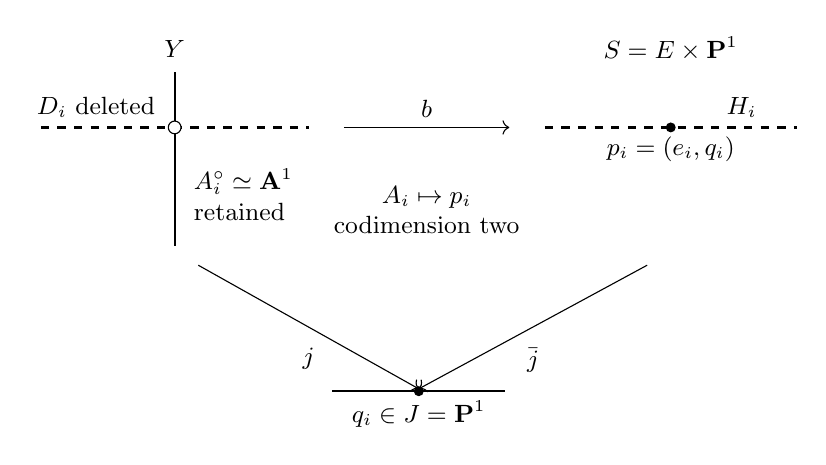
\begin{tikzpicture}[x=1cm,y=1cm,font=\small]
  \node at (0,2) {$Y$};
  \draw[dashed,thick] (-1.7,1)--(1.7,1);
  \node[above] at (-1,1) {$D_i$ deleted};
  \draw[thick] (0,-.5)--(0,1.7);
  \filldraw[fill=white] (0,1) circle (2.3pt);
  \node[right,align=left] at (.12,.15)
    {$A_i^\circ\simeq\AA^1$\\retained};
  \draw[->] (2.15,1)--(4.25,1) node[midway,above] {$b$};
  \node[align=center] at (3.2,-.05)
    {$A_i\mapsto p_i$\\codimension two};
  \node at (6.3,2) {$S=E\times\PP^1$};
  \draw[dashed,thick] (4.7,1)--(7.9,1);
  \fill (6.3,1) circle (1.8pt);
  \node[above] at (7.2,1) {$H_i$};
  \node[below] at (6.3,1) {$p_i=(e_i,q_i)$};
  \draw[->] (.3,-.75)--(3.1,-2.32)
    node[midway,below=4pt] {$j$};
  \draw[->] (6,-.75)--(3.1,-2.32)
    node[midway,below=4pt] {$\bar j$};
  \draw[thick] (2,-2.35)--(4.2,-2.35);
  \fill (3.1,-2.35) circle (1.8pt);
  \node[below] at (3.1,-2.35) {$q_i\in J=\PP^1$};
\end{tikzpicture}
\smallskip
\[
\begin{array}{c|c|c}
 & \text{multiplicity at }q_i & \text{boundary coefficient}\\ \hline
\text{direct base} & \min\{\infty,1\}=1 & 0\\
\text{iterated base} & \infty & 1
\end{array}
\]
\caption{Incidence schematic showing the two routes to the same point
$q_i$. The horizontal arrow is
the blowdown of complete surfaces: the retained $A_i^\circ$ maps to a
point on $H_i$. The hollow point $A_i\cap D_i$ is removed from $X$.
The divisor $A_i$ is omitted from the intermediate orbifold base because
$b(A_i)$ has codimension two in $S$, but contributes multiplicity one
to the direct base over $q_i$.}
\label{fig:retained-exceptional}
\end{figure}


\subsection{The models occurring before Claim 7.17}
We next check that this discrepancy occurs on the models used in the
cited claim. The \emph{relative core} used there has special general
fibres, and its base pair has general-type general fibres over $E$.
In our case it can be represented
by the identity of $Y$: the identity has point fibres, while the general
fibres of $(Y,D)\to E$ are the log-general-type punctured projective
lines. The identity is a neat and high model in the
terminology of \cite[Definitions 2.3 and Theorem 2.10]{CDHP2026}.
The log-canonical calculation \eqref{eq:log-canonical} gives the
Kodaira dimension one required in the subsequent reduction. General
Iitaka fibres are complete elliptic curves mapping isomorphically to
$E$.

An isogeny $E'\to E$ pulls the construction back to the blowup of
$E'\times\PP^1$ at all preimages of the centres. It is finite \'etale on
the entire pair. The boundary is the pullback of $D$, the exceptional
curves still have coefficient zero, and the log-canonical divisor is
still pulled back from $\OO_{\PP^1}(n-2)$. Thus the minimizing-isogeny
step in \cite[Equation (7.15.2)]{CDHP2026} leaves the relative-core
canonical dimension equal to one and retains the exceptional divisors.

For the birational contraction in \cite[Proposition 7.6]{CDHP2026},
we can take $b:Y\to S$. Indeed, the fixed semiabelian subvariety in
that construction is the image in $E$ of a general Iitaka fibre, hence
$E$ itself. The quotient is a point, and the resulting contracted
family is $\PP^1\times E\simeq S$. This product is smooth over all of $J$,
so the open set $J^0$ used for the smooth contracted family can be
taken to be $J$; its complement $\partial J$ is empty.
On the contracted
space $S$, the boundary $\sum_iH_i$ has the general-type orbifold base
shown in \eqref{eq:iterated-base}. This is consistent with
\cite[Claim 7.7]{CDHP2026}; the difficulty is transferring that
conclusion back to $(Y,D)$.

The proof next makes a birational change $J'\to J$ so that the main
component of $Y\times_JJ'$ is flat \emph{over $J'$}. Here
$j:Y\to\PP^1$ is already flat. One way to see this is that at each
point of the smooth curve base its local ring is a discrete valuation
ring, and the local rings of the dominant smooth integral source are
torsion-free modules over it. Torsion-free modules over a discrete
valuation ring are flat. A smooth birational model of the complete
curve $J=\PP^1$ is isomorphic to $J$. The choices in the proof can
therefore be instantiated with
\[
 J'=J,\qquad\bar X'=\bar X\times_JJ'=S,\qquad
 \widetilde X=S,\qquad\widetilde Y=Y.
\]
Here $\nu:\widetilde Y\to Y$ is the source modification and
$\mu:\widetilde X\to\bar X'$ is the resolution of the intermediate
target. Both are identities, and the maps to that target and to $J'$
are
\[
 \nu=\operatorname{id}_Y,\quad\mu=\operatorname{id}_S,\quad
 \widetilde c=b,\quad\widetilde j=\bar j.
\]
The boundary in \cite[Equation (7.16.7)]{CDHP2026} is then exactly $D$,
because there are no $\nu$-exceptional divisors to add.

\subsection{The change of flatness target}
Claim 7.17 asserts equality of the two divisors in
\eqref{eq:two-bases} on the resulting models. Its proof treats every
$\widetilde c$-exceptional divisor as having infinite boundary
multiplicity. To justify this, it uses flatness of
\[
 (Y\times_JJ')_{\mathrm{main}}\longrightarrow\bar X'
\]
although the preceding construction arranged flatness over $J'$.
These are different morphisms. In the displayed instance the former
map is the blowdown $b:Y\to S$. Its fibres are points away from the
centres and curves over the centres, so it is not flat. The divisors
$A_i$ are exceptional for $\widetilde c=b$ but are not exceptional for
$\nu=\operatorname{id}_Y$; they have boundary multiplicity $1$, not
$\infty$. Omitting them from the direct infimum is precisely what turns
\eqref{eq:direct-base} into the incorrect answer
\eqref{eq:iterated-base}.

This is a numerical failure of the asserted equality, as well as a
failure of the stated justification. Adding the $A_i$ to the boundary
would turn the blowdown into an orbifold morphism, but it would replace
$X$ by
\[
 E\times(\PP^1\setminus Q),
\]
which is not special and has group $\Z^2\times F_{n-1}$, where
$F_{n-1}$ is the free group of rank $n-1$.
Alternatively, making the intermediate target remember the blowups
retains the reducible fibres $D_i+A_i$ and restores the zero orbifold
base; the general-type base computed on the contracted model is then
lost. Neither modification establishes the original assertion for
the original open variety.

The counterexample and this calculation concern the fixed version
\cite{CDHP2026}. Its Theorem A is a separate assertion about linear
representation images. Our proof of that conclusion in
Section~\ref{sec:linear} uses independent inputs and does not use the
fibre-specialness assertion.

\section{The ordinary fundamental-group question}\label{sec:ordinary}

The monodromy theorem concerns every complex linear image, but does
not by itself determine the ordinary group. The remaining assertion
can be stated without representation-theoretic terminology.

\begin{question}\label{q:full}
For every connected smooth special complex quasi-projective variety
$V$, does $\pi_1(V)$ have a finite-index subgroup $H$ satisfying
$[H,[H,H]]=1$?
\end{question}

This is \cite[Conjecture 2.12]{CDHP2026}. The group is the ordinary
topological fundamental group; boundary meridians have not been
quotiented out. The surfaces in Theorem~\ref{thm:example} satisfy the
proposed conclusion and hence do not give counterexamples to it.

The precise obstruction to an inference from Theorem~\ref{thm:completion}
is faithfulness. Put $\Gamma=\pi_1(V)$ and write $\Gamma^{\un}$ for
its rational unipotent completion. The canonical homomorphism
$\Gamma\to\Gamma^{\un}(\Q)$ can have a kernel. The theorem sends
$\gamma_3\Gamma$ to the identity without identifying its elements in
$\Gamma$. For example, a finitely generated group with finite
abelianization has trivial rational unipotent completion, since a
nonzero nilpotent Lie algebra has nonzero abelianization. This
shows that a nontrivial group can be entirely invisible to rational
unipotent completion. The specialness hypotheses used here supply no
injectivity statement for the completion map.

A known group-theoretic reduction shows what an additional geometric
input could accomplish. If the full group $\pi_1(V)$ were virtually
solvable, Rogov's theorem would make it virtually nilpotent
\cite[Theorem C, Corollary 6.6]{Rogov2025}. A finitely generated
virtually nilpotent group has a torsion-free nilpotent subgroup $H$ of
finite index, and $H$ admits a faithful rational unipotent
representation by Mal'cev's theorem
\cite[Chapters 1 and 5; Chapter 6, p.~100]{Segal1983}.
The finite \'etale cover corresponding to $H$ is again special. The CDY
quasi-Albanese inputs from Section~\ref{sec:linear} therefore apply to
that cover, and Theorem~\ref{thm:completion} gives $[H,[H,H]]=1$.
Virtual solvability of the full ordinary group is not established by
the representation bounds.

Theorem~\ref{thm:example} also prevents an induction that requires the
general quasi-Albanese fibre itself to be special. Its fundamental
group is nonabelian free, while its image in the total group is zero.
Controlling that actual image is a different geometric problem.
The completion theorem addresses its image in every canonical
unipotent quotient; control of the kernel invisible to these quotients
remains necessary for Question~\ref{q:full}.


\begingroup
\small
\bibliographystyle{plain}
\bibliography{references}
\endgroup
\end{document}
